\chapter{Estimation Fundamentals}
\label{ch:estimation}

\begin{objectives}
\begin{itemize}
  \item Define estimators, bias, variance and mean-square error.
  \item Derive linear and weighted least squares, the covariance of their estimates, and the Gauss--Markov theorem.
  \item Understand maximum likelihood, Fisher information and the Cram\'er--Rao bound: what ``information'' means.
  \item Derive the minimum mean-square-error and linear minimum mean-square-error estimators, and the orthogonality principle.
  \item Derive recursive least squares, the Kalman filter without dynamics.
  \item See that, for linear-Gaussian problems, all of these approaches give the same answer.
\end{itemize}
\end{objectives}

Before filtering, which estimates a changing state from a stream of measurements, comes \emph{estimation}: inferring unknown quantities
from noisy data. This chapter develops the classical theory. Its punchline is that several quite different philosophies (minimize squared
errors; maximize the probability of the data; compute the posterior mean) lead to the same formulas for linear-Gaussian problems, and those
formulas are the Kalman update.

% ==============================================================================
\section{Estimators and their errors}

\subsection{The setting}

An unknown quantity $x \in \R^n$ is to be inferred from data $z \in \R^m$ related to it by a model, typically
\begin{equation}
  z = h(x) + n, \qquad n \text{ random, zero mean, covariance } R .
\end{equation}
An \term{estimator} is a function $\hat x(z)$ of the data. Because the data are random, the estimate is random too, and its quality is judged
by the statistics of its \emph{error} $e = \hat x - x$ over repetitions of the experiment.

\begin{definition}[Bias, covariance and mean-square error]
The \term{bias} of an estimator is $b = \E[\hat x] - x$; it is \emph{unbiased} if $b = 0$. Its \term{mean-square error} matrix is
$\E[ee\T]$, and its scalar mean-square error is $\E[\|e\|^2] = \tr\E[ee\T]$.
\end{definition}

\begin{proposition}[Bias--variance decomposition]
$\E[ee\T] = \Cov(\hat x) + bb\T$, and hence $\E\|e\|^2 = \tr\Cov(\hat x) + \|b\|^2$.
\end{proposition}
\begin{proof}
Write $e = (\hat x - \E\hat x) + b$ and expand; the cross terms vanish because $\E[\hat x - \E\hat x] = 0$.
\end{proof}

An estimator can be accurate in two ways: by being unbiased, and by having a small covariance. A filter reports a covariance $P$ along with its
estimate, and a \emph{consistent} filter is one whose reported $P$ equals its actual mean-square error matrix (\cref{ch:consistency}).

% ==============================================================================
\section{Linear least squares}
\label{sec:linear-ls}

\subsection{The estimate}

Consider the linear model
\begin{equation}
  z = Hx + n, \qquad \E[n] = 0, \quad \Cov(n) = R,
  \label{eq:linear-model}
\end{equation}
with $H \in \R^{m\times n}$ of full column rank ($m \ge n$). The \term{weighted least-squares} (WLS) estimate minimizes the residuals weighted by the
inverse noise covariance, so that reliable measurements count more:
\begin{equation}
  \hat x = \argmin_x\ (z - Hx)\T R\inv(z - Hx) = \big(H\T R\inv H\big)\inv H\T R\inv z .
  \label{eq:wls}
\end{equation}
The formula comes from setting the gradient $-2H\T R\inv(z - Hx)$ to zero (\cref{sec:least-squares}).

\begin{proposition}[Statistics of the WLS estimate]
\label{prop:wls-cov}
The WLS estimate is unbiased, and its covariance is
\begin{equation}
  \Cov(\hat x) = \big(H\T R\inv H\big)\inv .
\end{equation}
\end{proposition}
\begin{proof}
Write $\hat x = Lz$ with $L = (H\T R\inv H)\inv H\T R\inv$. Then $LH = I$, so $\hat x = x + Ln$ and $\E\hat x = x$. By \cref{prop:affine},
$\Cov(\hat x) = LRL\T = (H\T R\inv H)\inv H\T R\inv RR\inv H(H\T R\inv H)\inv = (H\T R\inv H)\inv$.
\end{proof}

The matrix $H\T R\inv H$ is the \term{information} that the measurements carry about $x$, and its inverse is the uncertainty of the estimate.
Information from independent measurements adds: with stacked blocks $z_i = H_ix + n_i$ and block-diagonal $R$,
$H\T R\inv H = \sum_iH_i\T R_i\inv H_i$.

\begin{worked}[fitting a line]
A target moves along a line with unknown initial position $p_0$ and velocity $v$, and its position is measured at times $t_1, \dots, t_m$ with
independent noise of standard deviation $\sigma$: $z_i = p_0 + vt_i + n_i$. With $x = (p_0, v)$, $H$ has rows $(1, t_i)$ and $R = \sigma^2I$, so
\begin{equation*}
  H\T R\inv H = \frac{1}{\sigma^2}\begin{bmatrix} m & \sum t_i \\ \sum t_i & \sum t_i^2 \end{bmatrix}.
\end{equation*}
For $m$ measurements equally spaced over a duration $T$ with times centered on zero, the off-diagonal terms vanish and the velocity variance is
$\sigma^2/\sum t_i^2 \approx 12\sigma^2/(mT^2)$: velocity is determined more precisely when the measurements span a longer time, a first glimpse of how
dynamics turn position measurements into velocity information (\cref{fig:lsfit}).
\end{worked}

\begin{figure}[t]
  \centering
  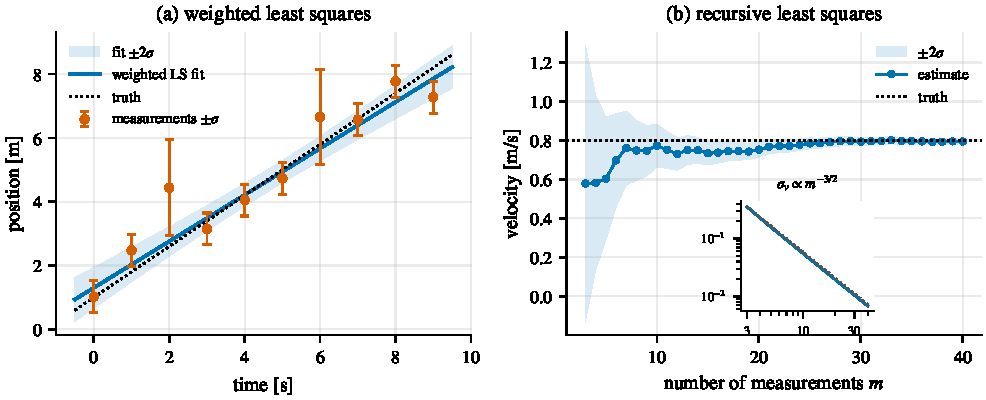
\includegraphics[width=\textwidth]{fig_lsfit.pdf}
  \caption{(a) Weighted least-squares fit of a line to noisy positions, with the $\pm2\sigma$ band of the fitted line from $(H\T R\inv H)\inv$.
  (b) Recursive least squares: the velocity estimate and its $\pm2\sigma$ bound as measurements arrive one at a time. The bound shrinks
  like $m^{-3/2}$ because later measurements also lengthen the time baseline.}
  \label{fig:lsfit}
\end{figure}

\subsection{The Gauss--Markov theorem}

Why weight by $R\inv$? Because it is the best possible linear choice.

\begin{theorem}[Gauss--Markov]
\label{thm:gauss-markov}
\index{Gauss--Markov theorem}
Among all linear unbiased estimators $\tilde x = Lz$ of $x$ in the model \eqref{eq:linear-model}, the WLS estimate \eqref{eq:wls} has the smallest
covariance: $\Cov(\tilde x) \succeq (H\T R\inv H)\inv$. It is the \term{best linear unbiased estimator} (BLUE).
\end{theorem}
\begin{proof}
Unbiasedness for every $x$ requires $LH = I$. Write $L = L_\star + D$ with $L_\star$ the WLS matrix; then $DH = 0$. The covariance is
$LRL\T = L_\star RL_\star\T + DRD\T + L_\star RD\T + DRL_\star\T$, and the cross terms vanish:
$L_\star RD\T = (H\T R\inv H)\inv H\T R\inv RD\T = (H\T R\inv H)\inv(DH)\T = 0$. So $\Cov(\tilde x) = \Cov(\hat x) + DRD\T \succeq \Cov(\hat x)$.
\end{proof}

The theorem needs no Gaussian assumption, only the first two moments of the noise. If the noise is Gaussian, more is true: WLS is the best of
\emph{all} unbiased estimators, linear or not, as the Cram\'er--Rao bound below shows.

% ==============================================================================
\section{Maximum likelihood}

\begin{definition}[Likelihood]
For a model with density $p(z\mid x)$, the \term{likelihood} of a value $x$ given observed data $z$ is $L(x) = p(z\mid x)$, viewed as a function of $x$.
The \term{maximum-likelihood} (ML) estimate maximizes it, equivalently minimizes the negative log-likelihood $-\log p(z\mid x)$.
\end{definition}

For Gaussian noise $n \sim \N(0, R)$ in $z = h(x) + n$,
\begin{equation}
  -\log p(z\mid x) = \tfrac12\big(z - h(x)\big)\T R\inv\big(z - h(x)\big) + \text{const},
\end{equation}
so ML estimation with Gaussian noise \emph{is} weighted least squares, linear or nonlinear. This is the justification of the least-squares
costs that pervade estimation, including the reprojection error of computer vision (\cref{ch:multiview}). For non-Gaussian noise, ML gives
other costs; heavy-tailed noise, for example, leads to the robust costs of \cref{ch:nlls}.

\subsection{Fisher information and the Cram\'er--Rao bound}

\begin{definition}[Fisher information]
\index{Fisher information}
For a model $p(z\mid x)$, the \term{Fisher information matrix} is
$\mathcal I(x) = \E\big[\nabla_x\log p(z\mid x)\,\nabla_x\log p(z\mid x)\T\big] = -\E\big[\nabla^2_x\log p(z\mid x)\big]$.
\end{definition}

The Fisher information measures how sharply the likelihood peaks around the true value: a likelihood that changes rapidly with $x$ pins $x$
down precisely. For the linear-Gaussian model, $\nabla^2_x\log p = -H\T R\inv H$, so $\mathcal I = H\T R\inv H$: the ``information matrix'' of WLS is the
Fisher information.

\begin{theorem}[Cram\'er--Rao lower bound]
\label{thm:crb}
\index{Cram\'er--Rao bound}
Under mild regularity conditions, every unbiased estimator satisfies $\Cov(\hat x) \succeq \mathcal I(x)\inv$.
\end{theorem}
\begin{proof}[Proof for a scalar parameter]
Let $s = \frac{\partial}{\partial x}\log p(z\mid x)$ (the \emph{score}). It has zero mean, since $\E[s] = \int\partial_xp\,\dd z = \partial_x\int p\,\dd z = 0$. Differentiating the
unbiasedness condition $\int\hat x(z)p(z\mid x)\,\dd z = x$ with respect to $x$ gives $\E[\hat x\,s] = 1$, hence $\Cov(\hat x, s) = 1$. By the
Cauchy--Schwarz inequality for covariances, $1 = \Cov(\hat x, s)^2 \le \Var(\hat x)\Var(s) = \Var(\hat x)\,\mathcal I(x)$.
\end{proof}

An unbiased estimator that attains the bound is \emph{efficient}. For the linear-Gaussian model, WLS attains it: $\Cov(\hat x) = (H\T R\inv H)\inv = \mathcal I\inv$.
No unbiased estimator can do better. This gives a precise meaning to the phrase used throughout these notes: \emph{information is inverse
covariance}, and independent measurements add their information.

% ==============================================================================
\section{Bayesian estimation}

\subsection{Priors and posteriors}

In the Bayesian view, the unknown $x$ is itself a random variable with a \emph{prior} density $p(x)$ that summarizes what is known before the
data. Bayes' rule gives the \emph{posterior} $p(x\mid z) \propto p(z\mid x)p(x)$, the complete description of what is known afterwards. Point estimates
summarize the posterior:
\begin{itemize}
  \item the \term{minimum mean-square error} (MMSE) estimate $\hat x = \E[x\mid z]$, the posterior mean;
  \item the \term{maximum a posteriori} (MAP) estimate, the posterior mode;
  \item and, ignoring the prior, the ML estimate.
\end{itemize}

\begin{theorem}[The conditional mean is optimal]
\label{thm:mmse}
Among all estimators $g(z)$, the conditional mean $\E[x\mid z]$ minimizes the Bayesian mean-square error $\E\|x - g(z)\|^2$, and indeed minimizes the
error matrix $\E[(x - g)(x - g)\T]$ in the Loewner order.
\end{theorem}
\begin{proof}
Fix $z$ and write $m = \E[x\mid z]$. For any value $g$, $\E\big[(x - g)(x - g)\T\mid z\big] = \Cov(x\mid z) + (m - g)(m - g)\T$ by the bias--variance decomposition
applied to the conditional distribution. The second term is PSD and vanishes exactly for $g = m$. Taking the expectation over $z$ preserves the
inequality.
\end{proof}

For a linear-Gaussian model the posterior is Gaussian (\cref{prop:map-ls}), so its mean and mode coincide: MMSE and MAP are the same estimate,
\begin{equation}
  \hat x = \big(P\inv + H\T R\inv H\big)\inv\big(P\inv\mu + H\T R\inv z\big), \qquad \Cov(x\mid z) = \big(P\inv + H\T R\inv H\big)\inv,
  \label{eq:bayes-linear}
\end{equation}
for a prior $\N(\mu, P)$. This is weighted least squares with one extra ``measurement'': the prior acts like a direct observation of $x$ with
value $\mu$ and covariance $P$. With an uninformative prior ($P\inv\to0$) it reduces to ML/WLS.

\subsection{Linear MMSE and the orthogonality principle}

The conditional mean can be hard to compute when distributions are not Gaussian. The best \emph{linear} (affine) estimator needs only means
and covariances.

\begin{theorem}[Linear minimum mean-square error estimator]
\label{thm:lmmse}
\index{linear MMSE estimator}\index{orthogonality principle}
Let $x$ and $z$ be random vectors with means $\mu_x$, $\mu_z$ and covariances $\Sigma_{xx}$, $\Sigma_{xz}$, $\Sigma_{zz} \succ 0$. Among estimators of the form
$\hat x = Az + b$, the mean-square error is minimized by
\begin{equation}
  \hat x = \mu_x + \Sigma_{xz}\Sigma_{zz}\inv(z - \mu_z),
  \qquad \E[(x - \hat x)(x - \hat x)\T] = \Sigma_{xx} - \Sigma_{xz}\Sigma_{zz}\inv\Sigma_{zx} .
\end{equation}
Its error is uncorrelated with the data: $\E\big[(x - \hat x)(z - \mu_z)\T\big] = 0$ (the \term{orthogonality principle}).
\end{theorem}
\begin{proof}
The error $e = x - Az - b$ has mean $\mu_x - A\mu_z - b$, which must vanish at the optimum (a non-zero mean only adds $bb\T$), so $b = \mu_x - A\mu_z$. Then
$e = (x - \mu_x) - A(z - \mu_z)$ and $\E[ee\T] = \Sigma_{xx} - A\Sigma_{zx} - \Sigma_{xz}A\T + A\Sigma_{zz}A\T$. Completing the square,
$\E[ee\T] = (A - A_\star)\Sigma_{zz}(A - A_\star)\T + \Sigma_{xx} - \Sigma_{xz}\Sigma_{zz}\inv\Sigma_{zx}$ with $A_\star = \Sigma_{xz}\Sigma_{zz}\inv$, which is minimal for $A = A_\star$. At the
optimum, $\E[e(z - \mu_z)\T] = \Sigma_{xz} - A_\star\Sigma_{zz} = 0$.
\end{proof}

The formulas are identical to Gaussian conditioning (\cref{thm:gauss-cond}): for jointly Gaussian variables the best linear estimator is the best
estimator of any kind, and for other distributions it is still the best linear one. The orthogonality principle has a geometric reading: the
estimate is the projection of $x$ onto the space of (affine) functions of the data, and the error is orthogonal to that space, exactly as a
least-squares residual is orthogonal to the column space (\cref{sec:least-squares}).

\paragraph{Application to the linear model.} For $z = Hx + n$ with prior mean $\mu$ and covariance $P$ for $x$, and noise uncorrelated with $x$:
$\mu_z = H\mu$, $\Sigma_{xz} = PH\T$, $\Sigma_{zz} = HPH\T + R$. \Cref{thm:lmmse} gives
\begin{equation}
  \hat x = \mu + K(z - H\mu), \qquad K = PH\T(HPH\T + R)\inv, \qquad \E[ee\T] = P - KHP .
  \label{eq:lmmse-update}
\end{equation}
This is the Kalman update (\cref{ch:kf}). By the Woodbury identity (\cref{thm:woodbury}) it equals \eqref{eq:bayes-linear}, but it requires
inverting an $m\times m$ matrix instead of an $n\times n$ one.

% ==============================================================================
\section{Recursive least squares}

Measurements often arrive one at a time, and recomputing \eqref{eq:wls} from scratch at each arrival would waste work. Since information adds,
the batch solution after $k$ measurements satisfies
\begin{equation}
  P_k\inv = P_{k-1}\inv + H_k\T R_k\inv H_k, \qquad P_k\inv\hat x_k = P_{k-1}\inv\hat x_{k-1} + H_k\T R_k\inv z_k,
\end{equation}
where $P_k$ is the covariance of $\hat x_k$. Rewriting this with the Woodbury identity gives the \term{recursive least squares} (RLS) update
\begin{equation}
  K_k = P_{k-1}H_k\T\big(H_kP_{k-1}H_k\T + R_k\big)\inv, \qquad
  \hat x_k = \hat x_{k-1} + K_k\big(z_k - H_k\hat x_{k-1}\big), \qquad
  P_k = (I - K_kH_k)P_{k-1} .
\end{equation}
Each step corrects the previous estimate by a gain times the \emph{innovation} $z_k - H_k\hat x_{k-1}$, the part of the new measurement that the old
estimate did not predict. It produces exactly the batch estimate at every step (\cref{fig:lsfit}b), at a cost that does not grow with the number
of measurements. RLS is the Kalman filter for a state that does not change; \cref{ch:kf} adds dynamics.

% ==============================================================================
\section{One answer, many derivations}

\begin{center}\small
\begin{tabularx}{\textwidth}{@{}l l >{\raggedright\arraybackslash}X@{}}
\toprule
Approach & Assumptions & Result for $z = Hx + n$ \\
\midrule
weighted least squares & second moments of the noise & $\hat x = (H\T R\inv H)\inv H\T R\inv z$ \\
Gauss--Markov (BLUE) & linear, unbiased & same \\
maximum likelihood & Gaussian noise & same \\
MAP / MMSE & Gaussian prior and noise & \eqref{eq:bayes-linear}: WLS with the prior as a measurement \\
linear MMSE & means and covariances only & \eqref{eq:lmmse-update}, equal to \eqref{eq:bayes-linear} \\
recursive LS & sequential data & same as batch, one measurement at a time \\
\bottomrule
\end{tabularx}
\end{center}

The Kalman filter inherits all of these interpretations. It is the exact Bayesian posterior for linear-Gaussian systems, the best linear
estimator when noises are merely uncorrelated, and a recursive least-squares solver. When models are nonlinear, these interpretations
separate, and the resulting approximations (\cref{ch:nlls,ch:nonlinear}) differ in which interpretation they try to preserve.

\begin{takeaways}
\begin{itemize}
  \item An estimator's error splits into bias and covariance: $\E[ee\T] = \Cov(\hat x) + bb\T$.
  \item Weighted least squares $\hat x = (H\T R\inv H)\inv H\T R\inv z$ has covariance $(H\T R\inv H)\inv$; information adds across independent measurements.
  \item Gauss--Markov: WLS with $R\inv$ weights is the best linear unbiased estimator.
  \item ML with Gaussian noise is least squares; the Fisher information bounds every unbiased estimator; information is inverse covariance.
  \item The conditional mean minimizes mean-square error; for Gaussians it equals the MAP estimate.
  \item The linear MMSE estimator $\mu + \Sigma_{xz}\Sigma_{zz}\inv(z - \mu_z)$ needs only second moments; its error is orthogonal to the data.
  \item Recursive least squares is the Kalman update without dynamics.
\end{itemize}
\end{takeaways}

\begin{exercises}
  \item Show that the sample mean of $m$ independent measurements of a scalar with variances $\sigma_i^2$ is not the BLUE unless all $\sigma_i$ are equal,
        and find the BLUE.
  \item For the line-fitting example with $m = 11$ measurements at $t = -5, \dots, 5$ and $\sigma = 1$, compute the covariance of $(p_0, v)$. How does it change
        if the times are $0, \dots, 10$? Interpret the off-diagonal term.
  \item Prove the matrix version of the Cram\'er--Rao bound for a linear-Gaussian model by computing $\nabla^2_x\log p$.
  \item Show that \eqref{eq:bayes-linear} and \eqref{eq:lmmse-update} agree, using \cref{thm:woodbury}.
  \item Derive the RLS update from the batch information form, and verify numerically that it reproduces the batch estimate at every step.
  \item Let $x \sim \mathcal U[-1, 1]$ and $z = x^3 + n$ with small Gaussian $n$. Compare the LMMSE estimate with the conditional mean, qualitatively. Why does
        the LMMSE estimate do poorly?
  \item A sensor reports a measurement with a bias $\beta$ that is not modeled. Show that the WLS estimate is biased by $(H\T R\inv H)\inv H\T R\inv\beta$, and explain
        why unmodeled biases are worse than large noise.
\end{exercises}
% Solutions to the exercises of Chapter 9.
\begin{solutions}
  \item The model is $z_i = x + n_i$, i.e.\ $H = \mathbf 1$ (a column of ones) and $R = \diag(\sigma_i^2)$. The WLS estimate is the BLUE
        (\cref{thm:gauss-markov}):
        \[
          \hat x = \big(\mathbf 1\T R\inv\mathbf 1\big)\inv\mathbf 1\T R\inv z = \frac{\sum_iz_i/\sigma_i^2}{\sum_i1/\sigma_i^2},
          \qquad \Var(\hat x) = \Big(\sum_i\frac{1}{\sigma_i^2}\Big)\inv,
        \]
        the inverse-variance weighted mean. The sample mean $\bar z = \frac1m\sum_iz_i$ is linear and unbiased with variance $\frac{1}{m^2}\sum_i\sigma_i^2$, and by the
        Cauchy--Schwarz inequality $\big(\sum_i\sigma_i^2\big)\big(\sum_i\sigma_i^{-2}\big) \ge m^2$, with equality only when all $\sigma_i$ are equal. So
        $\Var(\bar z) \ge \Var(\hat x)$, strictly unless the variances are equal: then (and only then) the two estimators coincide. One poor sensor can
        ruin a plain average; in the weighted one it simply counts for little.

  \item With $z_i = p_0 + vt_i + n_i$, $H$ has rows $(1, t_i)$ and $\Cov(\hat p_0, \hat v) = (H\T H)\inv$. For $t = -5, \dots, 5$, $\sum t_i = 0$ and $\sum t_i^2 = 110$, so
        \[
          (H\T H)\inv = \begin{bmatrix}11 & 0\\ 0 & 110\end{bmatrix}\inv = \diag\big(0.0909,\ 0.00909\big):
        \]
        $\sigma_{p_0} = 0.30$, $\sigma_v = 0.095$, uncorrelated. For $t = 0, \dots, 10$, $\sum t_i = 55$ and $\sum t_i^2 = 385$, and
        \[
          (H\T H)\inv = \frac{1}{1210}\begin{bmatrix}385 & -55\\ -55 & 11\end{bmatrix} = \begin{bmatrix}0.318 & -0.0455\\ -0.0455 & 0.00909\end{bmatrix}.
        \]
        The velocity variance is unchanged (it depends only on the spread of the times), but $p_0$ is now the value at the \emph{end} of the data,
        an extrapolation, with variance $3.5$ times larger and correlation $-0.85$ with $v$: a line that is too steep must start too low to pass
        through the data. The intercept is best determined at the centroid of the times, where the correlation vanishes.

  \item For $z = Hx + n$ with $n \sim \N(0, R)$, $\log p(z\mid x) = -\tfrac12(z - Hx)\T R\inv(z - Hx) + \text{const}$. Its gradient is
        $\nabla_x\log p = H\T R\inv(z - Hx)$ and its Hessian $\nabla_x^2\log p = -H\T R\inv H$, which does not depend on $z$, so
        $\mathcal I(x) = -\E[\nabla_x^2\log p] = H\T R\inv H$. (The outer-product definition agrees: $\E[H\T R\inv nn\T R\inv H] = H\T R\inv H$.) The matrix bound is
        proved like the scalar one: for an unbiased $\hat x$ and the score $s = \nabla_x\log p$, differentiating $\E[\hat x] = x$ gives $\Cov(\hat x, s) = I$, and
        the covariance matrix of $(\hat x, s)$,
        $\begin{bmatrix}\Cov(\hat x) & I\\ I & \mathcal I\end{bmatrix} \succeq 0$, has the PSD Schur complement $\Cov(\hat x) - \mathcal I\inv \succeq 0$ (Exercise 3.3's argument).
        WLS has covariance $(H\T R\inv H)\inv = \mathcal I\inv$ and attains the bound.

  \item Apply \cref{thm:woodbury} (as in Exercise 3.6) to the covariance of \eqref{eq:bayes-linear}:
        $(P\inv + H\T R\inv H)\inv = P - PH\T(HPH\T + R)\inv HP = P - KHP$ with $K = PH\T(HPH\T + R)\inv$, the covariance of \eqref{eq:lmmse-update}. For the mean,
        multiply out with this expression:
        \[
          (P - KHP)\big(P\inv\mu + H\T R\inv z\big) = \mu - KH\mu + \big(PH\T - KHPH\T\big)R\inv z .
        \]
        Since $K(HPH\T + R) = PH\T$, we have $PH\T - KHPH\T = KR$, so the last term is $Kz$, and the mean is $\mu + K(z - H\mu)$: the two forms agree.

  \item With prior $(\hat x_0, P_0)$, the batch estimate after $k$ measurements has information $P_k\inv = P_0\inv + \sum_{i\le k}H_i\T R_i\inv H_i$ and information
        vector $P_k\inv\hat x_k = P_0\inv\hat x_0 + \sum_{i\le k}H_i\T R_i\inv z_i$. Subtracting the expressions for $k - 1$ gives the recursion in information form
        stated in the chapter. Solving it for $\hat x_k$: $\hat x_k = P_k\big(P_{k-1}\inv\hat x_{k-1} + H_k\T R_k\inv z_k\big)$, and with
        $P_{k-1}\inv = P_k\inv - H_k\T R_k\inv H_k$ this is $\hat x_k = \hat x_{k-1} + P_kH_k\T R_k\inv(z_k - H_k\hat x_{k-1})$. Finally $P_kH_k\T R_k\inv = K_k$ (the
        push-through identity of Exercise 5.6) and $P_k = (I - K_kH_k)P_{k-1}$ by Woodbury. A numerical check with three unknowns, thirty scalar
        measurements of random variances and a weak prior: the RLS estimate and covariance agree with the batch solution after every
        measurement to $3\times10^{-12}$.

  \item The LMMSE estimate uses only second moments: with $\E[x] = \E[z] = 0$, $\Sigma_{xz} = \E[x^4] = \tfrac15$ and $\Sigma_{zz} = \E[x^6] + \sigma^2 = \tfrac17 + \sigma^2$,
        \[
          \hat x_{\mathrm{LMMSE}} = \frac{1/5}{1/7 + \sigma^2}\,z \approx 1.4\,z ,
        \]
        a straight line through a cube-root-shaped relation. The conditional mean $\E[x\mid z]$ follows the cube root, $\approx z^{1/3}$ wherever the noise is
        small compared with $z$. At $x = 0.5$ ($z = 0.125$) the LMMSE estimate is $0.17$, at $x = 0.9$ ($z = 0.73$) it is $1.02$, outside the support of $x$;
        the conditional mean gives $0.50$ and $0.90$. Overall, for $\sigma = 0.01$, the LMMSE root-mean-square error is $0.23$ against $0.075$ for the
        conditional mean (computed numerically). LMMSE does poorly because the dependence of $z$ on $x$ is strongly nonlinear: the best straight line
        fits neither small nor large values. This is the limitation the EKF inherits, mitigated by linearizing locally around the current estimate
        rather than globally.

  \item With $z = Hx + n + \beta$, the estimate $\hat x = Lz$ with $L = (H\T R\inv H)\inv H\T R\inv$ satisfies $LH = I$, so
        \[
          \hat x - x = Ln + L\beta, \qquad \E[\hat x] - x = (H\T R\inv H)\inv H\T R\inv\beta .
        \]
        The noise term has zero mean and covariance $(H\T R\inv H)\inv$, which shrinks as measurements accumulate ($\propto 1/m$ for $m$ comparable measurements).
        The bias term does not shrink: a constant offset in every measurement is averaged, not cancelled. The estimate therefore converges,
        with ever-smaller reported covariance, to the wrong value, and the filter becomes overconfident. Large noise is honest: it is in $R$, so it
        makes the covariance large. An unmodeled bias is invisible to the covariance and, if $\beta$ lies in the range of $H$, invisible in the residuals
        too, because it is indistinguishable from a different $x$. The cure is to model the bias as a state (\cref{ch:processes}), which is exactly
        why IMU biases are part of the filter state.
\end{solutions}

